\section{The \rnn{} algorithm}%
\label{sec:neuralringer}


Instead of using electron shower-shape variables~\cite{TRIG-2018-05} to discriminate between electrons and background, the Neural-Ringer algorithm uses another construction to represent the shower information, referred to here as 'Rings'. These are transverse energy rings, built from sums of calorimeter-cell energies, around each candidate provided as an RoI by the L1 trigger. The distribution of those energy sums is used by a set of neural networks to distinguish electrons from background. This section describes the Neural-Ringer algorithm.


\subsection{Building the rings}\label{ssec:rnn_for_online_and_eletrons}


Since the Neural-Ringer algorithm was designed to operate online in software at the \fastcalo{} stage, approximations were made. Specifically, rectangular rings are constructed to match the grid layout of the calorimeter cells, and the ring coverage is bounded by the RoI's area. The granularity changes in different regions of the detector are neglected in order to design an algorithm that uses a cell grid defined as a number of cells in the ($\eta$,$\phi$) directions so that the $\eta\times\phi$ region where the rings are built is not exactly constant along the full detector. This effect is mostly relevant for the EM1 layer where the $\eta$-granularity used by the algorithm is 0.003 for  $0<|\eta|<1.81$, 0.004 for $1.81<|\eta|<2.01$ and 0.006 for $2.01<|\eta|<2.37$.




The algorithm's RoI covers a calorimeter region of $0.4\times0.4$ in the $\eta\times\phi$ plane, centred on the L1-provided RoI. 
The algorithm starts at the EM2, where the $\eta\times\phi$ position of the cell with the highest \ET in the RoI is taken as the centre of the cascade interaction in the calorimeter. This initial seed-cell position is propagated to other calorimeter layers in order to define the axis of the rings in those layers. Then, for each layer, the algorithm refines the seed position by searching for the most energetic cell inside a reconstruction window of $0.1\times0.1$ in the $\eta\times\phi$ plane centred on the EM2 initial seed, and the energy deposition of an incoming particle is extracted by building concentric rings of cells, simply referred to as \enquote{rings}. 

\begin{figure}[h!t]
	\centering
	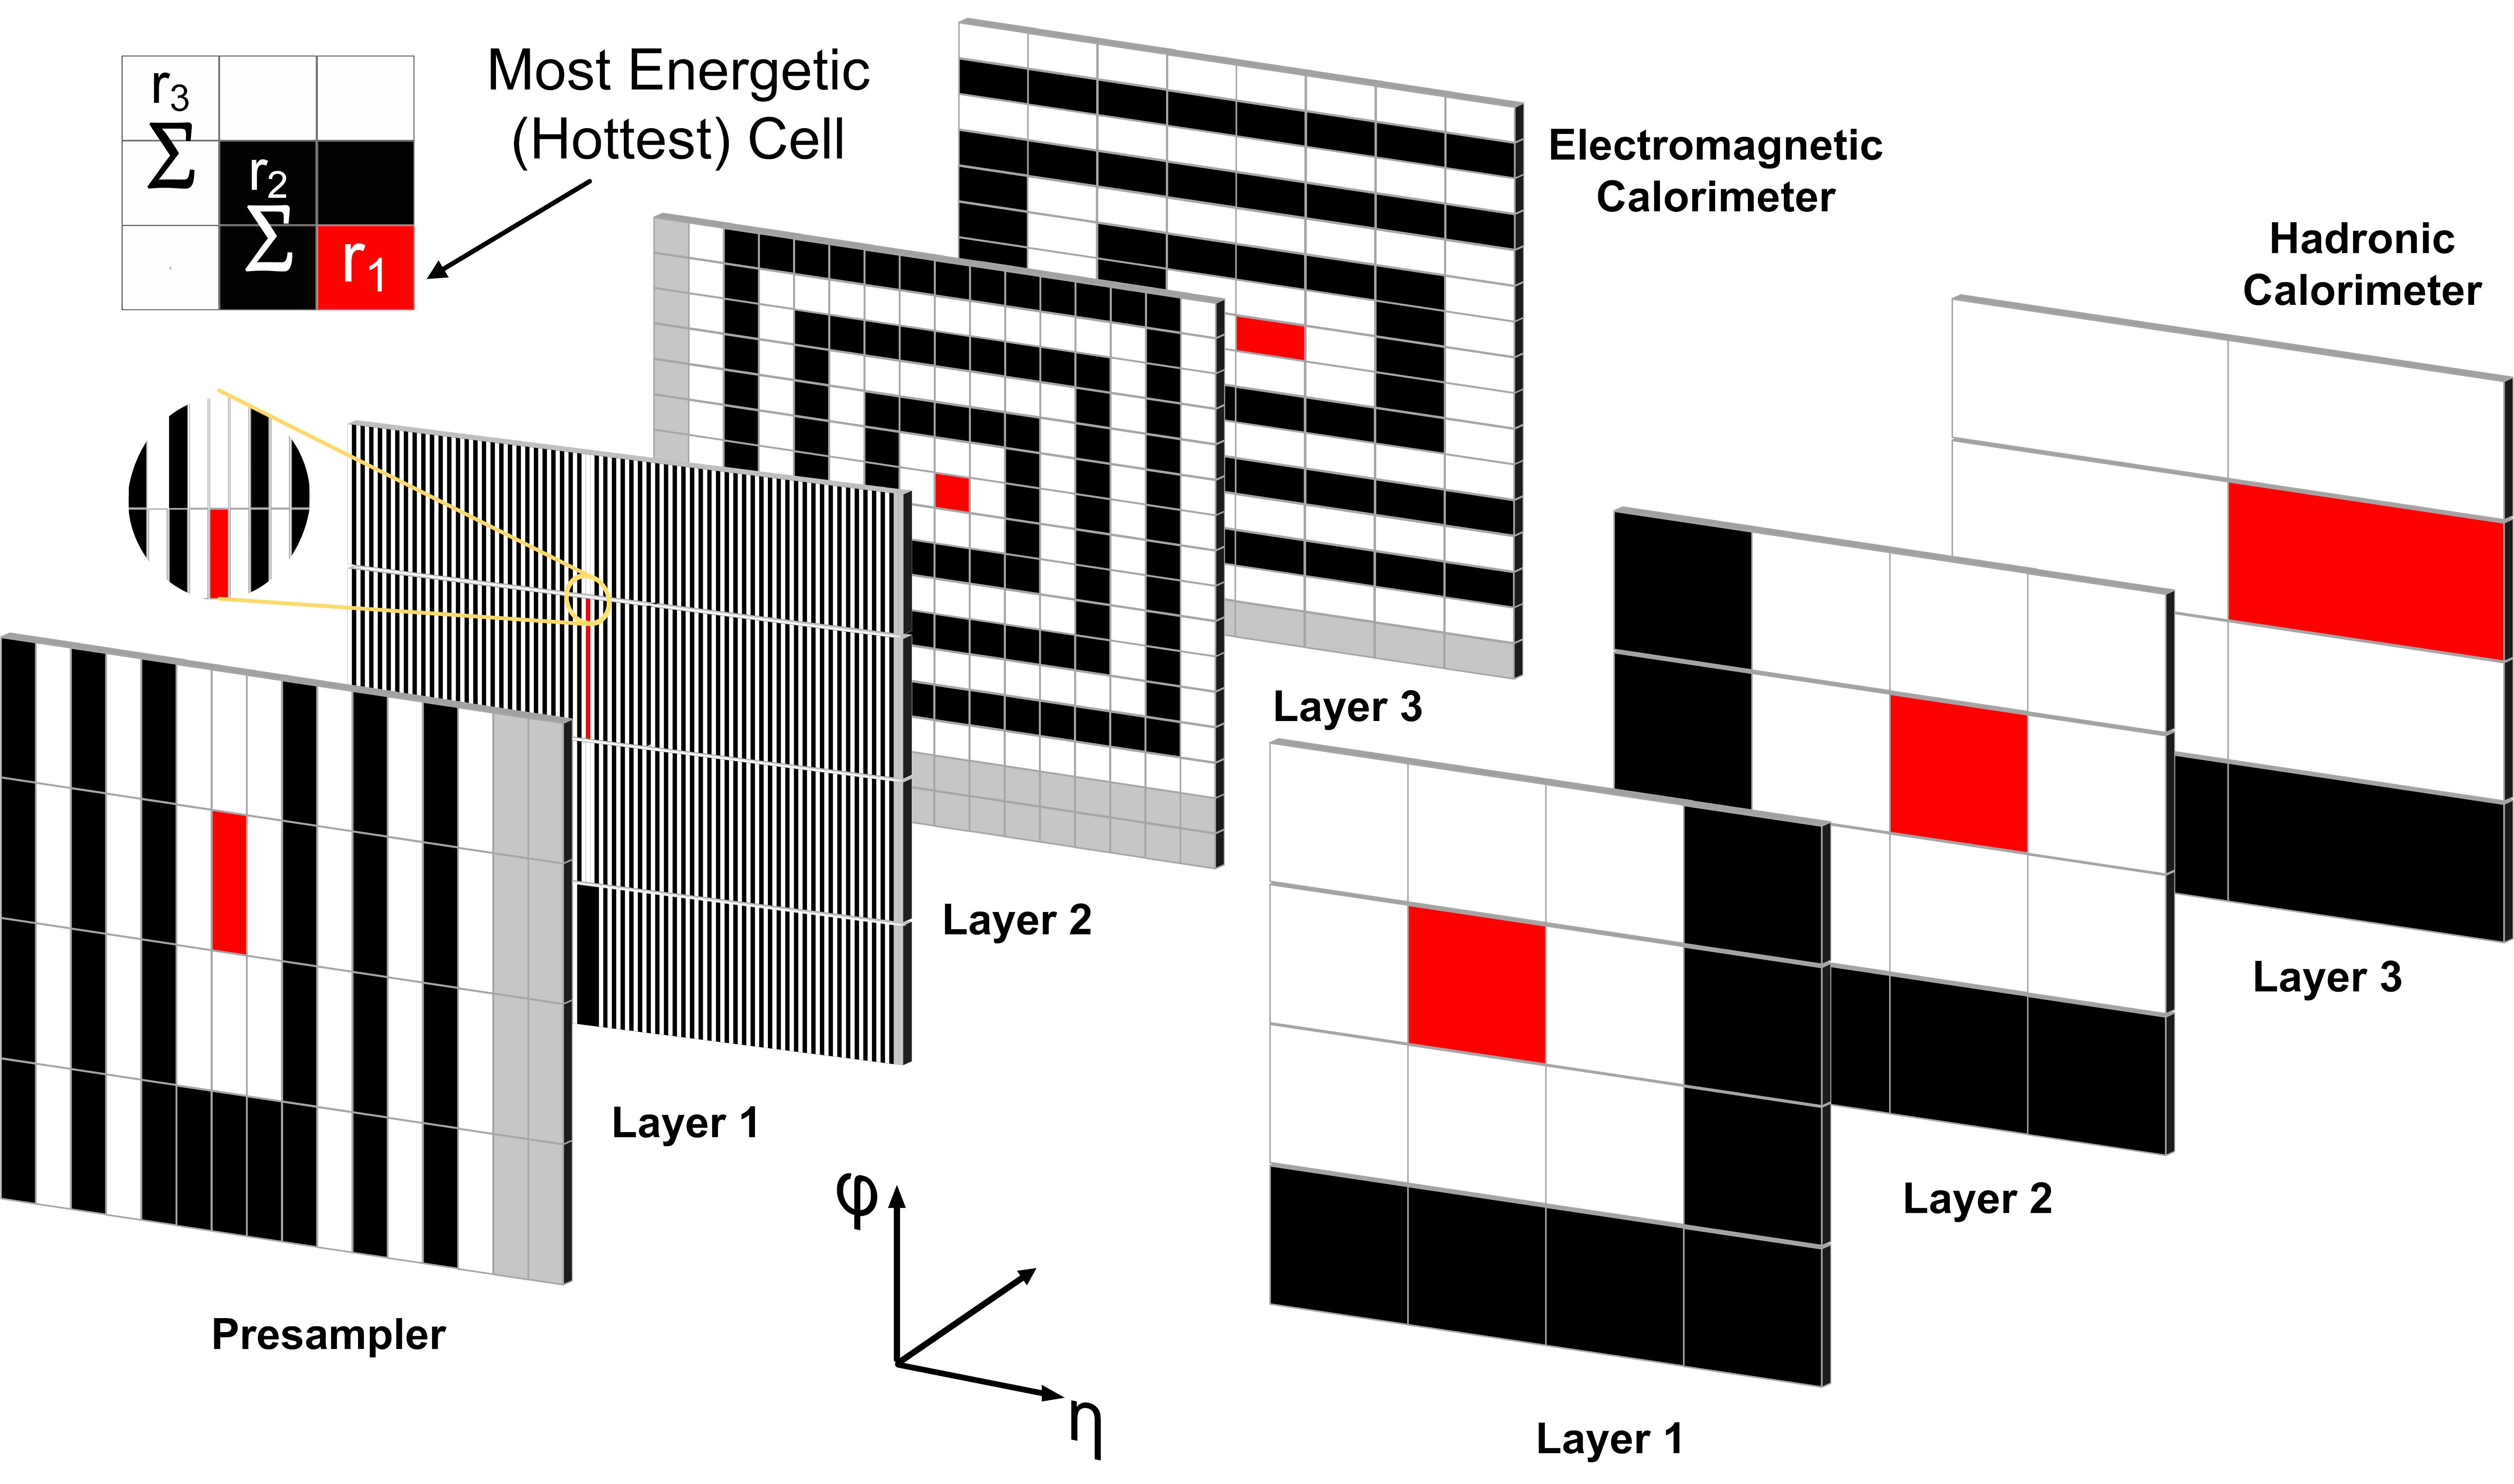
\includegraphics[width=0.8\textwidth]{sections/03_ringer/figures/ATLAS_Layers_V4.png}
	\caption{\label{fig:calo_rings}
		Sketch illustrating the ring-shaped energy description.
		The most energetic cell is in red, while the consecutive neighbouring rings are represented by alternating grey and black cells. Extracted from~\cite{TRIG-2018-05}.    
	}
\end{figure}




The refined seed ($c_{\text{hot},l}$) is used as the starting point to build the rings. A ring $R_{n,l}$ contains all $c_{n,l}$ cells in calorimeter layer $l$ which are $n$ cells away from the refined seed (\figurename~\ref{fig:calo_rings} shows the parameters used for each layer.). Formally,


\begin{equation*}
%\label{eq:ring_idx}
R_{n,l} = \left\{c_{n,l} \mid n = \left\lfloor \max{\left( 
\frac{| \eta_{i,l} - \eta_{\text{hot},l} |}{h_{\eta,l}}, 
\frac{| \phi_{i,l} - \phi_{\text{hot},l} |}{h_{\phi,l}} 
\right)} \right\rceil, 
\forall c_{i,l} \in
\Theta_{\text{RoI},l}
\right\},
\end{equation*}



\noindent where $\eta_{i,l}$, $\phi_{i,l}$
and $\eta_{\text{hot},l}$, $\phi_{\text{hot},l}$ are respectively the $c_{i,l}$ and $c_{\text{hot},l}$
cells' positions in $\eta$ and $\phi$ plane; $h_{\eta,l}$ is the $l^{\text{th}}$ layer's cell size in $\eta$; $h_{\phi,l}$ is the $l^{\text{th}}$ layer's cell size in $\phi$; $\Theta_{\text{RoI},l}$ is the set of cells
in the $l^{\text{th}}$ layer which are within the Ringer RoI; and $\lfloor \cdot \rceil$ is the \textit{round} function.
\tablename~\ref{tab:ring_alg_parameters} shows the number of rings computed at each layer and the respective granularity.

\input{sections/03_ringer/tables/granularity}

The sums of the transverse energies of cells $c_{n,l}$ in the rings $R_{n,l}$ form a vector of discriminating quantities. They are ordered laterally outwards and longitudinally from the innermost to outermost layer of the calorimeter, thus providing the ring-shaped information about the RoI.

The ring-building process results in a total of 100 rings across all calorimeter layers in each RoI. Well-known features of EM shower physics allow a large reduction in dimensionality to be achieved by compacting the typical input space of approximately 1000--1200 cells per RoI into these 100 rings: the rings can keep a complete description of the longitudinal and symmetric lateral information. 
%However, the algorithm only approximates this concept in order to meet the online operation requirements and avoid further manipulation of the instrumental information. 
Figure~\ref{fig:rings_profile} shows the expected ring profile produced by  electrons and QCD jets.



\begin{figure}[!ht]
  \centering
  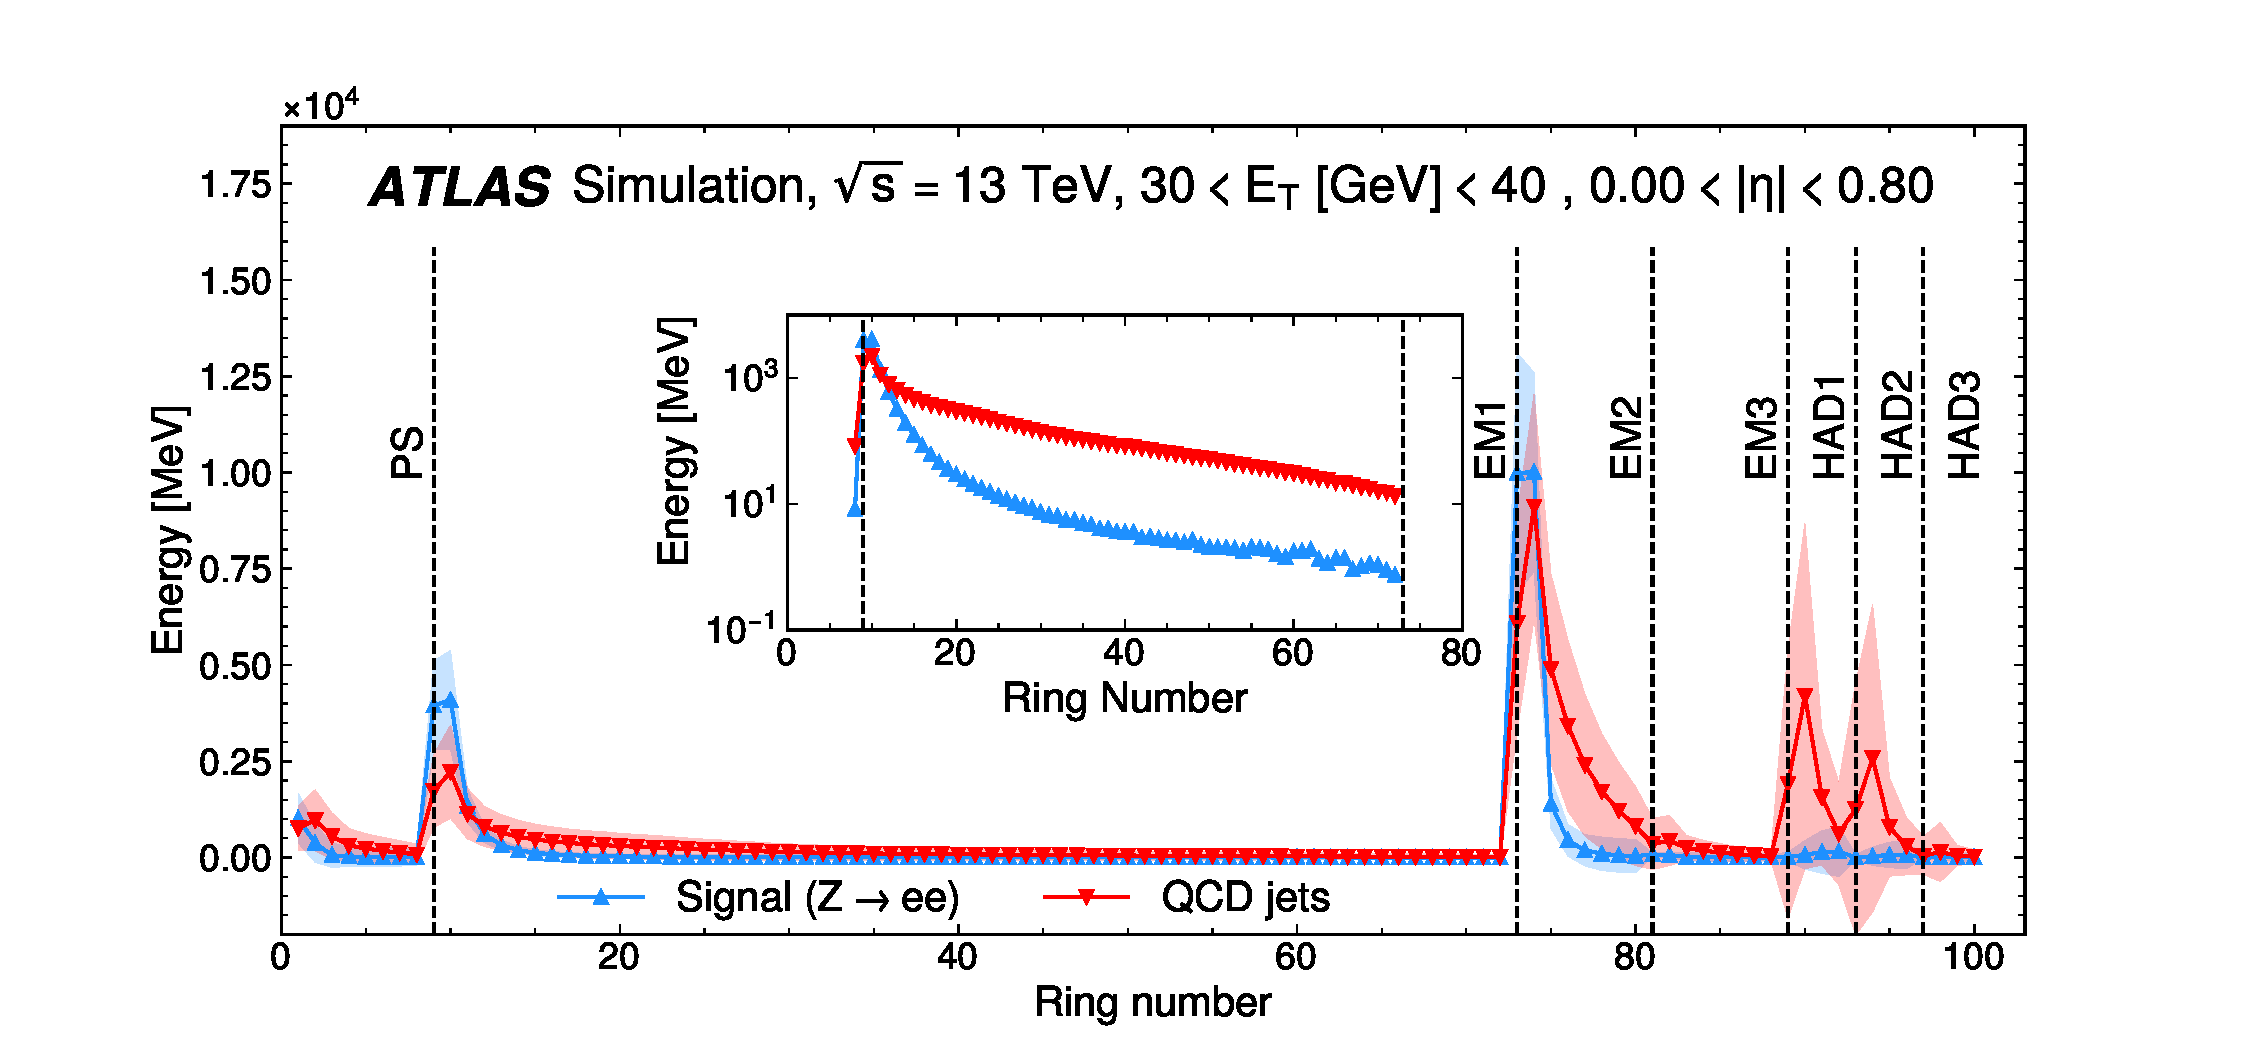
\includegraphics[width=0.9\textwidth]{sections/03_ringer/figures/ring_shape.pdf}
  \caption{ Simulated average ring profiles for jets and electrons in the bin $30 \leq \ET < 40$~GeV and $0.0 \leq \eta < 0.8$ for each layer of the calorimeter. The profile in the inset shows the EM1-layer ring energies on a logarithmic scale. 
  Almost all the energy of the electrons is absorbed by the electromagnetic layers and no energy deposit is expected in the hadronic calorimeter. Instead, a significant fraction of the jet energy is absorbed by the hadronic layers and only a part of it is absorbed by the electromagnetic calorimeter.
  The shaded area indicates the standard deviation of each ring energy.}
  \label{fig:rings_profile}
\end{figure}

\subsubsection{Ring sums as discriminating variables}

All rings are concatenated into a single vector of 100
variables. The variables are normalized to the absolute value of the total RoI energy, as shown in Eq.~(\ref{eq:ring_norm}):

\begin{equation}
  r^\prime_{k} = \frac{r_{k}}{| \sum\limits_{i=1}^{100} r_i
  |}, \;\;\;
    \forall \; k\in\{1,\dots,100\},
\label{eq:ring_norm}
\end{equation}

where $r_k$ or $r_i$ is the sum of transverse energy of the cells in the ring with index $k$ or $i$, and $r^\prime_{k}$ is the normalized ring value with index $k$.
The absolute value is used because of negative noise accumulation from some cells within the reconstruction window that were not excited by the particle shower.  This procedure was initially proposed and examined in Ref.~\cite{1995_seixas_ringer} as a way of preserving the shower energy profile as fractions of the total energy. 


\subsection{Motivation for using a set of neural networks}\label{ssec:nn_set}

The normalized concatenated vector of rings is fed into a set of multi-layer perceptrons (MLPs) trained individually for a particular region of \eteta space, where $E_T$ is the transverse energy of the electron candidate and $|\eta|$ is its impact position in the calorimeter. The model used to process a specific EM shower is the one trained for the \eteta region where it belongs.

For calorimetry, the use of a set of models, each specific to a particular phase-space region, mitigates fluctuations in the variables' profiles
due to differences in shower energy and detector response.
A large contribution comes from discrete detector-granularity changes in the phase space. Other important factors 
influencing such profiles are the
amount of the detector material as a function of \abseta{} and the dependence of the
underlying shower-development processes on the incoming
particle's energy. Although the latter changes are mostly continuous, it is also
possible to approach the problem via space discretization.

At the hardware resource level, splitting the training into multiple small models to accommodate detector response inhomogeneities speeds up the training cycle and allows data to be handled in memory, since only a small portion of the data is used to train a specific model. Limiting the memory required for tuning the models was of particular interest in order to benefit from low-memory processing nodes, as these were the ones mostly available in the Worldwide LHC Computing Grid~\cite{2015_lcg_tdr} during the model developments process effort.\@ In addition, the decomposition of the problem can also lead to a reduction in training time~\cite{Polikar2006}, as observed heuristically
%\footnote{When using NVIDIA RTX 2080Ti in tensorflow 1.14 and a minibatch size of 1024, a MLP with single hidden layer, a substantial increase in the runtime (from 4 to 41 seconds per epoch) with respect to the set version was observed.} 
when comparing the tuning time of the set with that of a single overall model. 
%With regard to operation, the proposed set only requires the choice of a single model in order to operate, whereas the more common committee-machine approaches require the computation of different models to run in parallel with a fusion method~\cite{zhou_ensemble}.
Therefore, the chosen set configuration adds
minimal overhead in terms of trigger latency. Similarly, our choice was to
use low-complexity models, with a single hidden layer and few neurons, to develop a method competitive with the cut-based approach in terms of processing speed.






\subsection{Data selection for 2017 and 2018 operation}

The training procedure for 2017 operation was based on samples of simulated $Z\rightarrow e^+e^-$ decays, selected with a $Z\rightarrow e^+e^-$ \tnp method~\cite{TRIG-2018-05}, and 
QCD dijet background events, both generated with Pythia 8.186. 
For the \tnp method in a $Z\rightarrow$ decay, one of the electrons candidates must satisfy the Tight identification criteria, the tag, while the second electron candidate, the probe, is lated used to train the set of neural networks of the ringer algorithm. 
For simulated QCD dijet samples, a filter was applied to enrich them with particles produced in the hard scatter with a summed transverse energy exceeding 17~GeV in a region of $\Delta\eta\times\Delta\phi=0.1\times0.1$.
Both $Z\rightarrow e^+e^-$ and hadronic jets from QCD hard scatter simulated samples included an average of 60 pileup interactions per bunch crossing,
covering running conditions of full Run-2.

After the training stage, threshold values for the discriminating variables must be determined in order to select good electron candidates. Since the thresholds obtained in simulation caused efficiency losses at the end of the HLT due to differences in the model responses between collision data and simulation, new values were obtained using probe electrons selected by the $Z\rightarrow e^+e^-$ \tnp method from the full set of 13~TeV collision data \textit{pp} recorded by ATLAS in 2016, which also satisfied the electron Tight offline criteria available.


For background, objects rejected by the $Z\rightarrow e^+e^-$ \tnp method, which do not belong to any tag--probe electron pair, were used if they were also rejected by the electron Loose offline criteria. During 2016 data-taking, pileup reached 40 interactions per bunch crossing.

For 2018 operation, a purely data-driven strategy was used, selecting events from the 2017 recorded collision data to train the models and adjust all thresholds. To be used for tuning and analysis, the recorded collision data were first required to pass the standard ATLAS data quality procedure as explained in~\cite{DAPR-2018-01}. 


\subsection{Training and decision making for 2017 and 2018 operation}\label{sec:tuning}


The 2017 procedure derived a specific MLP model for each region of \eteta phase space, using simulated samples, and defined threshold values for the discriminating variables by using 2016 collision data and targeting a signal efficiency similar to that of the cut-based trigger. The training procedure and decision-making processes were the same for all phase-space regions. For the \rnn{}, each MLP is an expert model for a single phase-space region, containing its own topology and parameters.

The model parameters were optimized using events selected from simulation datasets. 
The structure consists of a single fully-connected hidden layer, which may contain from 5 to 20 hidden units, an input layer with 100 inputs, one for each ring, and an output layer with a single neuron. 
The activation function for both the hidden and output neurons is a hyperbolic tangent, which has often been  used in MLP designs~\cite{haykin_2008}. 

To assess the statistical fluctuations of the efficiency measurements with respect to the model parameters obtained from the training procedure, the stratified $k$-fold cross-validation method~\cite{haykin_2008}, with $k=10$, was used, although repeating the training and testing procedures on different randomly chosen subsets increased the computational cost. 
The stratified $k$-fold is one of the most common cross-validation techniques and consists of partitioning the dataset into $k$ disjoint subsets, each model being tested with the $i^\text{th}$ subset after being trained with the other ones. The dataset stratification follows the empirical order of the event selection, in order to allow straightforward job parallelization, i.e.\ random permutation is not employed. 

For each cross-validation sort and working point, 100 networks, initialized as in~\cite{initnw}, are optimized by back-propagating the mean squared error through the RPROP algorithm~\cite{rprop}. This repeated model initialization seeks to avoid poor sub-optimal solutions due to the use of gradient-based algorithms.
For each training procedure, only three models out of the 100 are retained: two for retrieving the best efficiency when fixing the sensitivity or false positive probabilities to the baseline \fastcalo{} efficiency and another that gives the maximum $SP$ value. 

The maximum SP is the value that best relates the balance between signal detection probability and the probability of fake signal in the ROC curve (i.e., the knee of the curve) and is defined as:

\begin{equation*}
SP = \sqrt{\sqrt{P_\text{D}(1-F_\text{A})}\cdot\frac{P_\text{D} + (1-F_\text{A})}{2}}
\end{equation*}


\noindent where $P_\text{D}$ is the signal detection probability (or sensitivity) and $F_\text{A}$ is the probability of a fake signal (false positive). 
An early stopping~\cite{haykin_2008} technique is employed to avoid model over-training. The selection of the optimal iteration and operating model is based on a heuristic approach (multi-stop)~\cite{Goodfellow2016}.


Computational resources were used to tune 1.3 million shallow-learning neural networks, which resulted in a set of \SI{20}{MLPs} for each one of the four working points used by electron triggers in the HLT. 
The training strategy for 2017 data-taking considered only four regions in $|\eta|$ ($0.0\rightarrow 0.8\rightarrow1.37\rightarrow1.57\rightarrow2.47$) and five regions in \ET ($15~\GeV\rightarrow 20~\GeV\rightarrow 30~\GeV\rightarrow 40~\GeV\rightarrow 50~\GeV\rightarrow\infty$).
Apart from few exceptions, the models in the set employ five neurons in the hidden layer. 

After the training stage, decisions are made by applying a threshold requirement to the one-dimensional output node of each expert MLP. 
As in the HLT likelihood \cite{aaboud2019electron} algorithm, the threshold value used in the \rnn algorithm is computed as a linear function of \avgmu{}, the mean number of pileup interactions per bunch crossing.
However, non-linear behaviour was observed near the asymptote of the output activation function (see Figure~\ref{fig:nn_correction_with_tansig}) when using the \enquote{medium} or \enquote{tight} operating point. It was 
observed that this behaviour can be avoided by replacing the hyperbolic tangent activation function in the output neuron with a linear function (Figure~\ref{fig:nn_correction_without_tansig}) for operation after the training stage is completed.
This strategy ensures linear behaviour of the targeted\footnote{same signal detection probability of the online precision electron LH algorithm, increased by a factor of 50\%, for each one of the four trigger operation points.} signal efficiency with respect to the online pileup estimator, similar what was used in \cite{aaboud2019electron}. 
To account for Monte Carlo and collision data mis-modelling (see Figure~\ref{fig:nn_mc15_vs_data16}), the parameters of the linear threshold correction were derived using 2016 collision data and an upper bound of $\avgmu=40$ pileup interactions (i.e.\ the corrected threshold value is constant for pileup values above the upper bound).


\begin{figure}[h!tb]
  \begin{center}
  %\hspace{0.01\textwidth}
  \begin{subfigure}[c]{.48\textwidth}
  \centering
  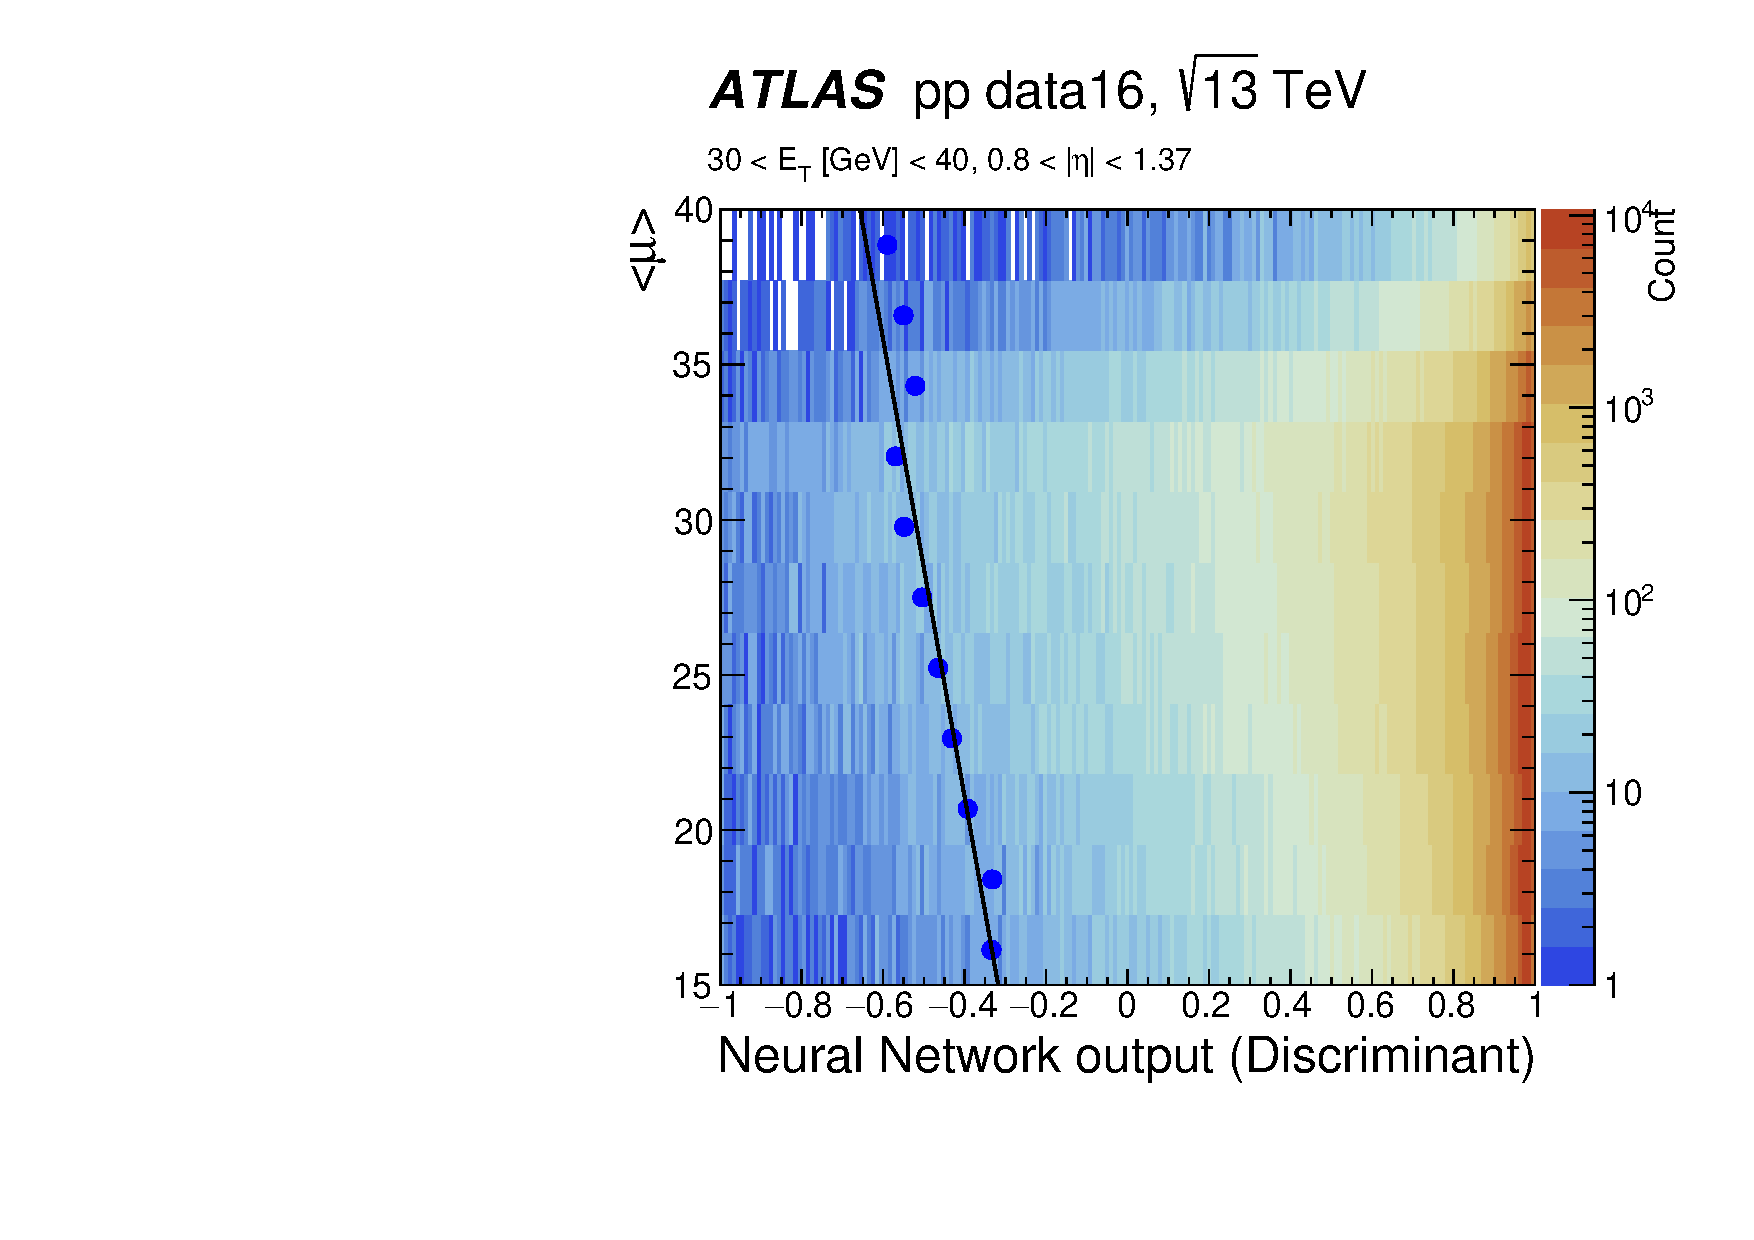
\includegraphics[width=\textwidth]{sections/03_ringer/figures/nn_output_versus_mu_with_tanh.pdf}
  \caption{MLP output with a hyperbolic tangent activation function in the output neuron versus pileup.}
  \label{fig:nn_correction_with_tansig}
  \end{subfigure}
  \hfill
  \begin{subfigure}[c]{.48\textwidth}
  \centering
  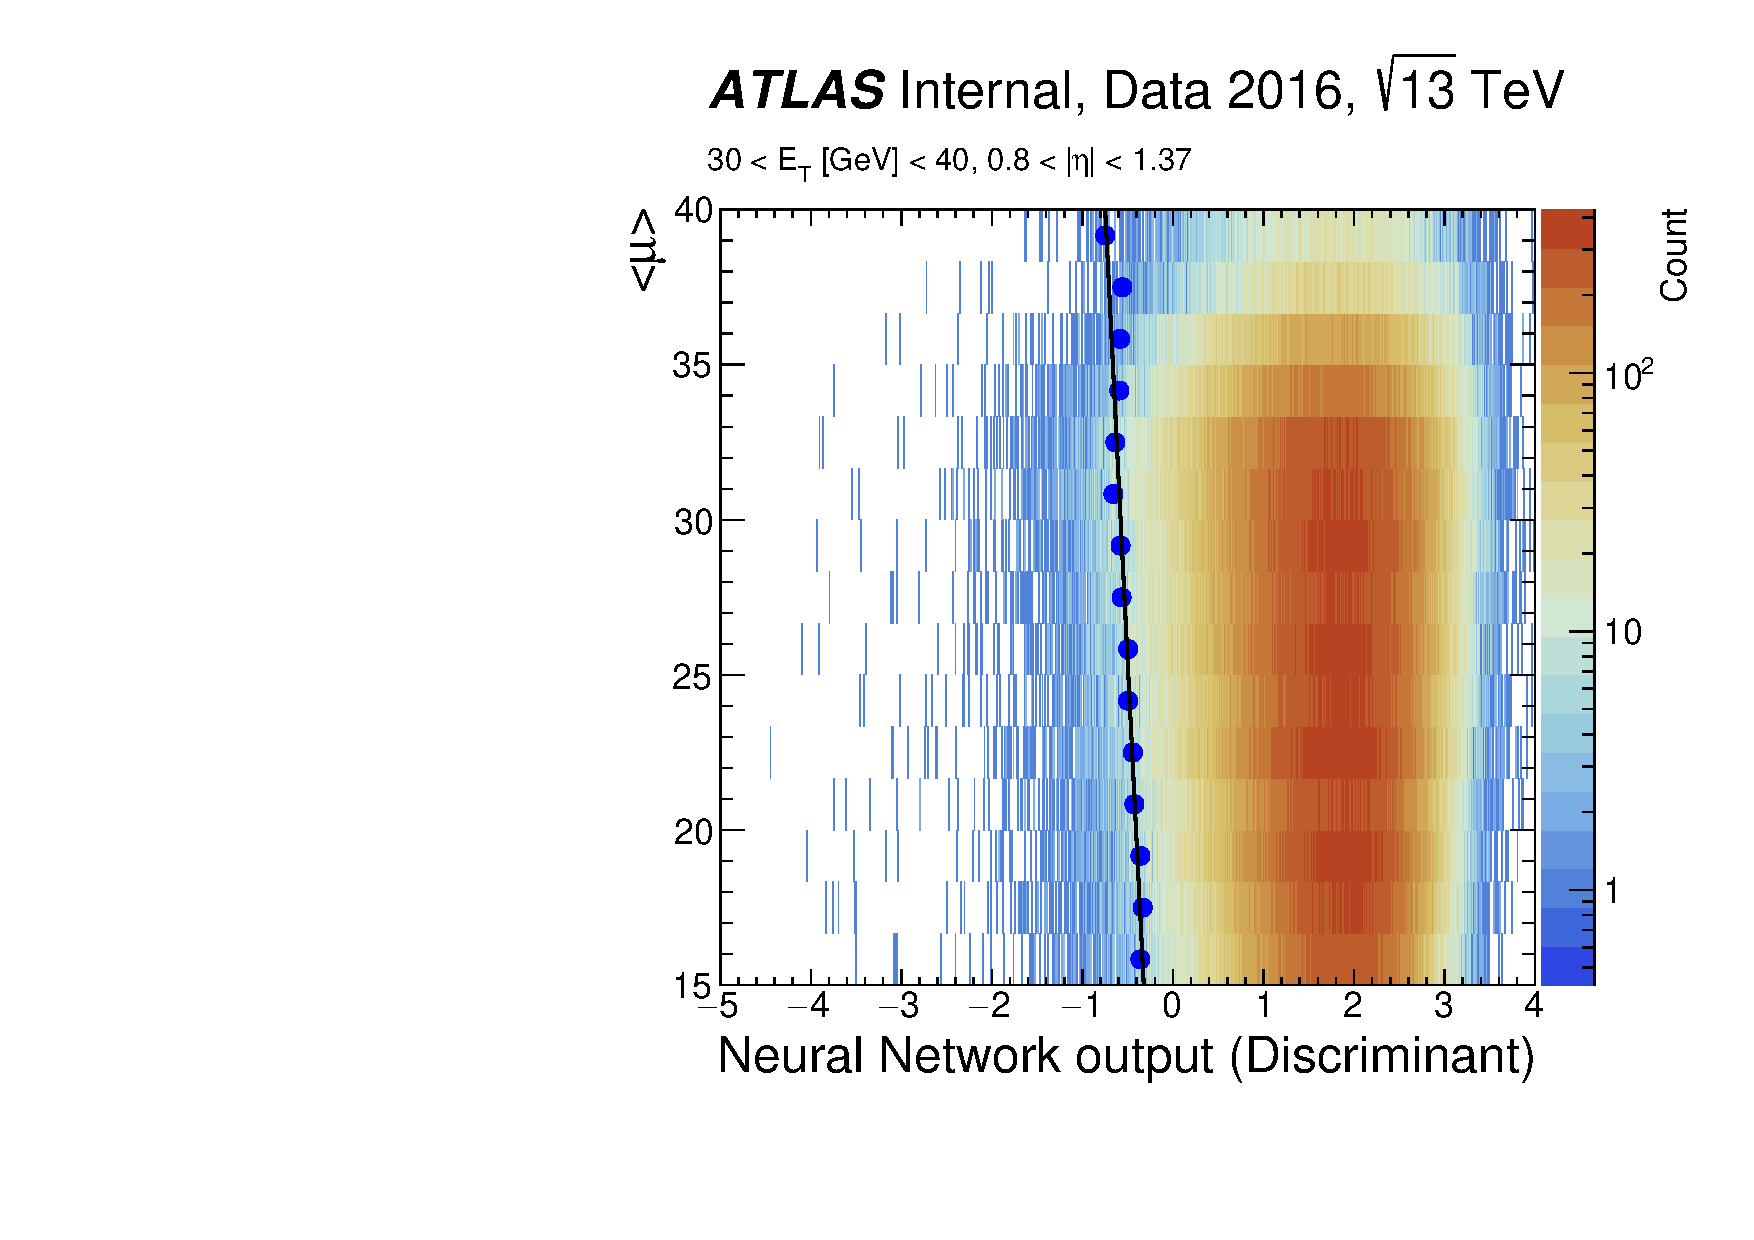
\includegraphics[width=\textwidth]{sections/03_ringer/figures/nn_output_versus_mu.pdf}
  \caption{MLP output with a linear activation function in the output neuron versus pileup.}
  \label{fig:nn_correction_without_tansig}
  \end{subfigure}
  %\hfill
  \caption{
    \rnn output as a function of pileup, \avgmu, for $Z\rightarrow ee$ probes in 
    2016 collision data selected using the training criteria.
    The computed threshold per \avgmu{} unit for achieving the targeted 
    efficiency is shown as a full blue circle. The black line is a linear fit to the thresholds.
    The output space is computed using the trained model without modifications in (a), 
    while in (b) the activation function in the output neuron is replaced with a linear function.
  }%
  \end{center}
\end{figure}

\begin{figure}[!ht]
  \centering
  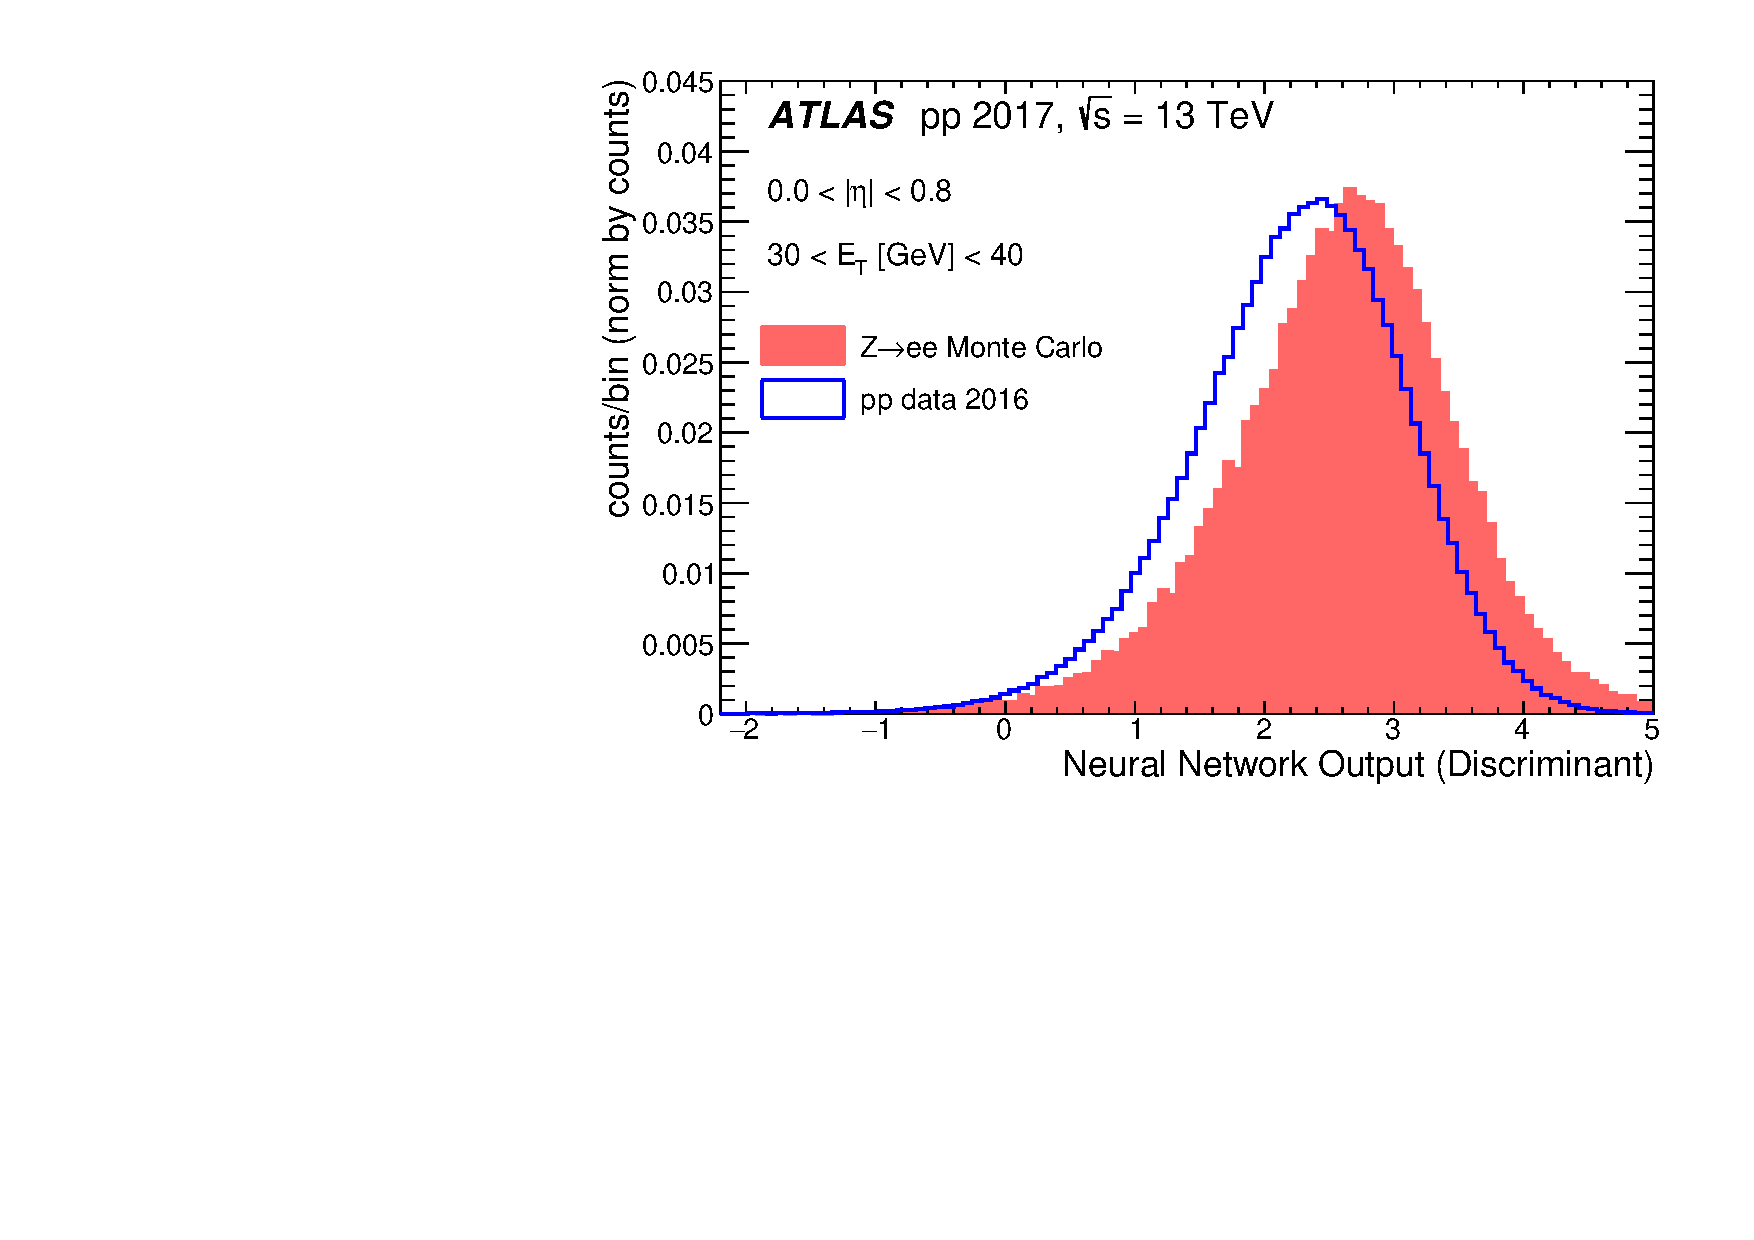
\includegraphics[width=0.7\textwidth]{sections/03_ringer/figures/nn_output_mc15_versus_data16_et2_eta0.pdf}
  \caption{Differences between simulation samples (filled histogram) and collision data (empty histogram) obtained in 2016 $Z\rightarrow ee$ \tnp{} for one region of the phase space.
  The comparison is made between the normalized distributions of the output of the neural network (the discriminant) obtained for these two cases. 
  The shift in discriminant value between simulation and collision data is caused by differences between the simulation and data rings used as input
  to the model. }
  \label{fig:nn_mc15_vs_data16}
\end{figure}


It was observed
that the rings in the region $2.37<\abseta<2.47$ had particular profiles due to
the lack of EM1 cells in this region and required a specific discriminant threshold in order to keep the signal efficiencies close to those of the cut-based triggers. In order to avoid retraining all models, it was decided to split the last $|\eta|$ region in two, from $1.37\rightarrow 2.47$ to $1.37\rightarrow2.37\rightarrow2.47$, and duplicate all models, for this region, to the new bin. Finally, the set operated in 2017, which combines every $\eta$ boundary with each \ET boundary, has a total of 25 MLP models. The set's boundaries are defined in Table~\ref{tab:ensemble_regions}.

\input{sections/03_ringer/tables/ensemble}

On the other hand, the 2018 training procedure employed a single set structure for all working points and used the 2017 collision data, selected with  \Zee{} \tnp{} event selection, for training, as was the case for the derivation of the offline and final \hlt likelihood models~\cite{PERF-2017-01}. 
Most of the procedure was kept unchanged for 2018. The developments for 2018 data benefited from the data conditions being similar to those in 2017. To simplify the training strategy, the selection of three models for each training was abandoned, keeping only the maximum $SP$ model, as the previous approach was more complex without a clear increase in trigger efficiency. 

Likewise, MLPs with 5 to 10 units in the hidden layer were tuned, as most models did not require more than 10 units in 2017. The training optimizer was changed to \emph{Adam}~\cite{kingma2014adam}, instead of RPROP, and the MLP model topology was modified to have a hidden layer with fully connected neurons, with rectified linear units (RELU) as the activation function, and an output layer with one neuron using a sigmoid activation function. Specialized MLPs were implemented in the region $2.37<\abseta<2.47$, where different ring profiles were observed before 2017 operation, resulting in the operation of \SI{25}{MLPs}. Finally, the upper bound for threshold corrections was set to $\avgmu{}=100$~pileup interactions in order to extrapolate the operation of the models to a never-reached pileup level. 





